%%%%%%%%%%%%%%%%%%%%%%%%%%%%%%%%%%%%%%%%%%%%%%%%%%%%%%%%%%%%%%%%%%%%%%%%%%%%%%%%%%%%%%%%%
%%%%%%%%%%%%%%%%%%%%%%%%%%%%         PRELIMINARY DESIGN        %%%%%%%%%%%%%%%%%%%%%%%%%%
%%%%%%%%%%%%%%%%%%%%%%%%%%%%%%%%%%%%%%%%%%%%%%%%%%%%%%%%%%%%%%%%%%%%%%%%%%%%%%%%%%%%%%%%%
\section{Preliminary Design} % (20 Points)
\label{sec:PreliminaryDesign}
% Section Requirements
% 1) Describe design/analysis methodology
% 2) Document design/sizing trades
% 3) Describe/document methodology for prediction of aircraft performance (include capabilities and uncertainties)
% 4) Provide estimates of the aircraft lift, drag and stability characteristics and method of prediction
% 5) Provide estimates of the aircraft mission performance 


\subsection{Methodology}
\label{ssec:methodology}


%----------------
%---   Preliminary design methodology flow chart
%----------------
\begin{figure}[h!]
	\centering
	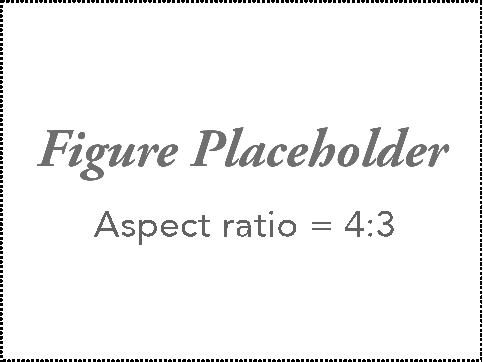
\includegraphics[width=3in]{draft4x3}
	\caption{Preliminary design process flow chart.}
	\label{fig:prelimdesflow}
\end{figure}



\subsubsection{Quantify Basic Constraints}
\label{sssec:constraints}

The sensitivity study presented in \cref{ssec:SensitivityStudy} did not include any constraints, but rather simple sensitivities that informed our conceptual design choices.  To begin a preliminary design, we first needed to translate the given constraints (listed in \cref{ssec:MissionReqs}) into mathematical formulas for rapid comparison and trade studies. Aside from the obvious constraints (such as the wing span constraint), we determined the following to be important expressions.

\paragraph{Stall Speed}

\[V_\text{stall} = \left[ \frac{2W}{\rho S_\text{ref} C_{L_\text{max}}} \right]^{1/2}\]

Where \(V_\text{stall}\) is the stall speed, \(W\) is the total aircraft weight, \(\rho\) is the ambient air density, \(S_\text{ref}\) is the reference wing area, and \(C_{L_\text{max}}\) is the maximum aircraft lift coefficient.

\paragraph{Take-off Distance}

\[ d_{LO} = \frac{ W^{5/2} }{ \left( \rho S_\text{ref} C_{L_\text{max}} \right)^{3/2} P_\text{net} } \]
Where \(d_{LO}\) is the distance to lift-off, \(P_\text{net}\) is the net power, that is, the power accounting for both thrust and drag, and the other variables are as defined previously.

\paragraph{Maximum Speed}

\[ V_\text{max} = \left[ \frac{ \frac{T_a}{S_\text{ref}} + \frac{W}{S_\text{ref}}\sqrt{\left(\frac{T_a}{W}\right)^2 - 4C_{D_0}K } }{\rho C_{D_0}} \right]^{1/2} \]

Where \(V_\text{max}\) is the maximum velocity, \(T_a\) is the available thrust, \(C_{D_0}\) is the zero-lift drag coefficient of the aircraft, and \(K\) is an empirical constant assumed here to be 0.38.

\paragraph{Maximum Range}

\[R = \frac{e_b}{g} \eta \frac{L}{D} \frac{m_b}{m_\text{tot}}\]

Where \(R\) is the total range; \(e_b\) is the battery energy per unit mass; \(g\) is the gravitational constant; \(\eta\) is the combination of efficiency factors from the battery, motor, and propeller (\(\eta=\eta_b\eta_m\eta_p\)); \(L/D\) is the aircraft lift to drag ratio, and \(m_b/m_\text{tot}\) is ratio of the battery mass to total aircraft mass.

\paragraph{\(C_L\) for Maximum Efficiency (and Range)}

\[C_{L_\text{max L/D}} = \left[ C_{D_p} \pi S_\text{ref} Re \right]^{1/2}\]

Where \(C_{D_p}\) is the parasitic drag coefficient for the aircraft, \(Re\) is the Reynolds number, and other variables are defined previously.


\paragraph{Climb Rate}

\[ v_z = \frac{V_\infty \left(T - D\right)}{W}\]

Where \(v_z\) is the vertical climb rate, \(V_\infty\) is the flight velocity of the aircraft, \(T\) is the thrust force magnitude, and \(D\) is the drag force magnitude.


\paragraph{Coordinated Turn Radius}

\[r_\text{turn} = \frac{V^2}{g \tan\phi}\]

Where \(r_\text{turn}\) is the turn radius, \(V\) is the aircraft speed, and \(\phi\) is the bank angle of the aircraft.

\paragraph{Coordinated Turn Load Factor}

\[n = \frac{1}{\cos\phi}\]

Where \(n\) is the load factor.

\subsubsection{Analysis Models}


\paragraph{Weight Estimation}


\paragraph{Propulsion Model}


\paragraph{Vortex Lattice Method (XFLR5, AVL, or VLM.jl)}


\paragraph{Structures Stuff (Beams, composites, etc.)}


\paragraph{Code}




\subsection{Trade Studies}
\label{ssec:tradestudies}

\begin{equation}
	\label{eqn:optdef}
	\begin{aligned}
		\text{maximize}: 
		& ~~M2 + M3 \\
		\text{with respect to}:
		& ~~W, S_\text{ref}, C_{D_0}, \text{\color{\BYUred} [PAYLOAD STUFF]}, P_a \\
		\text{subject to}: 
		& ~~V_\text{stall}, V_\text{maneuver}, d_{LO}, R, r_\text{turn}
	\end{aligned}
\end{equation}

where \(V_\text{maneuver}\) is the maximum velocity boundary associated with structural failure due to maneuver acceleration.


\subsubsection{Wing/Tail Design}

\paragraph{Airfoil(s)}

\begin{figure}[h!]
	\centering
	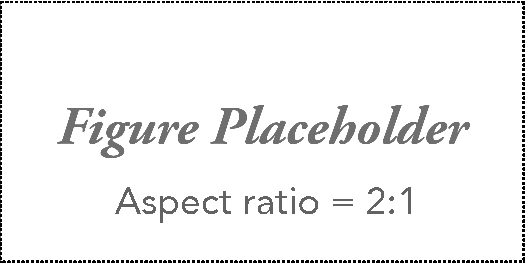
\includegraphics[width=5in]{draft2x1}
	\caption{Airfoil geometry comparison.}
	\label{fig:airfoilgeometrycomp}
\end{figure}

\begin{figure}[h!]
	\centering
	\begin{subfigure}[b]{0.475\textwidth}
		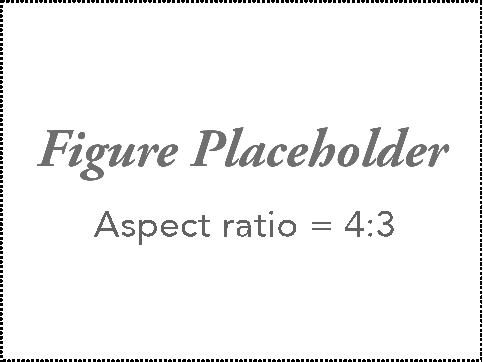
\includegraphics[width=\textwidth]{draft4x3}
		\caption{\(c_\ell\) vs \(\alpha\)}
		\label{fig:clva}
	\end{subfigure}
	%
	\begin{subfigure}[b]{0.475\textwidth}
		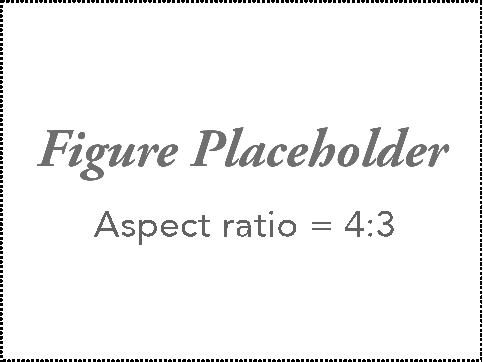
\includegraphics[width=\textwidth]{draft4x3}
		\caption{\(c_\ell\) vs \(c_d\)}
		\label{fig:clvcd}
	\end{subfigure}
	\caption{Airfoil Polar comparison.}
	\label{fig:airfoilpolarcomp}
\end{figure}



\paragraph{Sizing}


%----------------
%---   Preliminary wing and tail sizes.
%----------------
\begin{table}[h!]
	\centering
	\caption{Preliminary wing and tail sizes.}
	\label{tab:prelimwingsize}
	\rowcolors{2}{BYUbluelite}{white}
	\begin{tabular}{ C{1in}  C{1in}  C{1in}  C{1in}}
		
		\rowcolor{BYUbluemid}
		Parameter & Wing & Vertical Tail & Horizontal Tail \\
		
		Span (ft) & & &\\
		
		Root Chord (ft) & & &\\
		
		Tip Chord (ft) & & &\\
		
		Wing Area (ft\(^2\)) & & &\\
		
		Aspect Ratio & & &\\
		
	\end{tabular}
\end{table}


%----------------
%---   Preliminary lift distribution plot (superimpose all missions)
%----------------
\begin{figure}[h!]
	\centering
	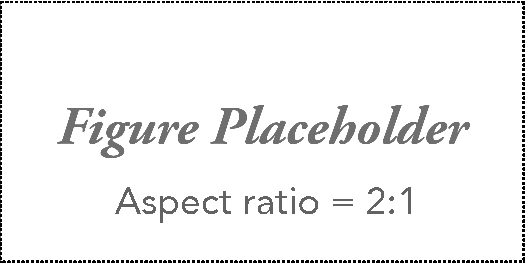
\includegraphics[width=5in]{draft2x1}
	\caption{Lift distribution at cruise for each mission.}
	\label{fig:prelimliftdist}
\end{figure}

\subsubsection{Propulsion}

%----------------
%---   Preliminary propulsion system selection
%----------------
\begin{table}[h!]
	\centering
	\caption{Preliminary propulsion system comparison.}
	\label{tab:prelimpropselection}
	\rowcolors{2}{BYUbluelite}{white}
	\begin{tabular}{ C{1in}  C{0.25in}  C{1in}  C{0.5in}  C{0.75in}  C{0.75in}  C{0.75in}}
		
		\rowcolor{BYUbluemid}
		Motor & Kv & Battery & Current (Amps) & Propeller & Static Thrust (lbs) & Total Weight (lbs) \\
		
		& & & & & & \\
		
		& & & & & & \\
		
		& & & & & & \\
		
	\end{tabular}
\end{table}


%----------------
%---  Motor/Prop efficiency curves
%----------------
\begin{figure}[h!]
	\centering
	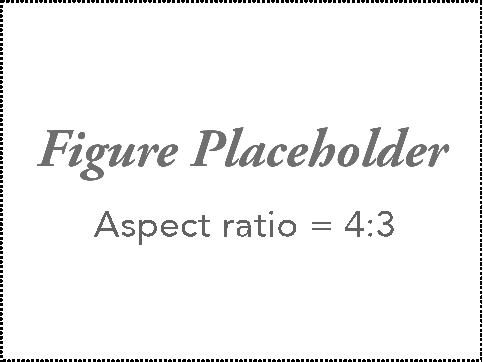
\includegraphics[width=3.5in]{draft4x3}
	\caption{Efficiency curves for the motor and propeller selection.}
	\label{fig:propefficiency}
\end{figure}



\subsubsection{Fuselage}



\subsubsection{Payload}

\subsubsection{\color{\BYUred} [OTHER TRADE STUDIES TO FIND THE ANSWER TO THE OPTIMIZATION PROBLEM.]}



\subsection{Estimated Aircraft Performance}
\label{ssec:estaircraftperfomance}


\subsubsection{Performance Prediction Methodologies and Uncertainties}
\label{sssec:uncertaintyanalysis}



\subsubsection{Lift and Drag}
\label{sssec:liftdrag}

%----------------
%---   Estimated Lift and Drag values
%----------------
\begin{table}[h!]
	\centering
	\caption{Estimated total lift and drag values.}
	\label{tab:estimatedLD}
	\rowcolors{2}{BYUbluelite}{white}
	\begin{tabular}{ C{1in}  C{1in}  C{1in}  C{1in}}
		
		\rowcolor{BYUbluemid}
		Parameter & Mission 1 & Mission 2 & Mission 3 \\
		
		\(C_{L_\text{max}}\) & & &\\
		
		\(C_{L_\text{avg}}\) & & &\\
		
		\(C_{D_0}\) & & &\\
		
		\(L/D_\text{cruise}\) & & &\\
		
		Efficiency Factor (e) & & & \\
		
	\end{tabular}
\end{table}


\paragraph{Lift Analysis}


\paragraph{Drag Analysis}

%----------------
%---   Drag breakdown for each mission (use stacked bar charts, not pie charts.)
%----------------
\begin{figure}[h!]
	\centering
	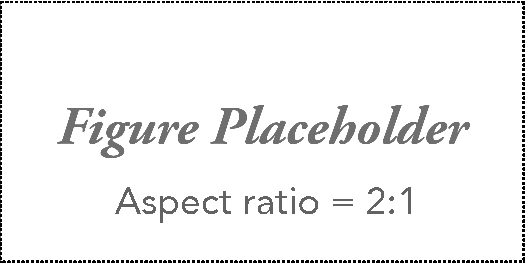
\includegraphics[width=5in]{draft2x1}
	\caption{Drag breakdown for each mission}
	\label{fig:dragbreakdown}
\end{figure}


\subsubsection{Stability}
\label{sssec:stability}

%----------------
%---   Longitudinal Static Stability  (should mention static margin when talking about this plot.)
%----------------
\begin{figure}[h!]
	\centering
	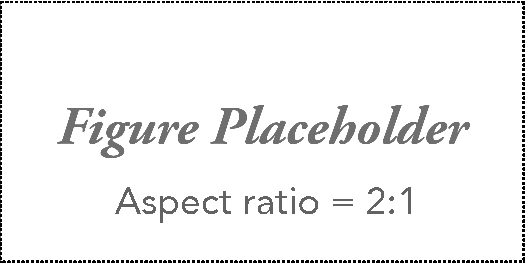
\includegraphics[width=5in]{draft2x1}
	\caption{Moment coefficient vs \(\alpha\)}
	\label{fig:cmva}
\end{figure}

%----------------
%---  M1 Stability Derivatives (these are not control derivatives)
%----------------
\begin{table}[h!]
	\centering
	\caption{Stability derivatives for Flight Mission 1.}
	\label{tab:stabilityderivatives1}
	\rowcolors{2}{BYUbluelite}{white}
	\begin{tabular}{ B{1in} ? C{3em} C{3em}?C{3em} C{3em}?C{3em} C{3em}?C{3em} C{3em}?C{3em} C{3em} }

	\rowcolor{BYUbluemid}

	\cellcolor{white} & Angle of Attack & \(V_{TO}\)/ \(V_C\) & Side Slip Angle & \(V_{TO}\)/ \(V_C\) & Roll Rate & \(V_{TO}\)/ \(V_C\) & Pitch Rate & \(V_{TO}\)/ \(V_C\) & Yaw rate & \(V_{TO}\)/ \(V_C\)  \\

	Lift  Force &  \(C_{L_{\alpha}}\) & 0.0000/ 0.0000 & \(C_{L_{\beta}}\) & 0.0000/ 0.0000 & \(C_{L_{p}}\) & 0.0000/ 0.0000 & \(C_{L_{q}}\) & 0.0000/ 0.0000 & \(C_{L_{r}}\) & 0.0000/ 0.0000 \\

	Drag  Force & \(C_{D_{\alpha}}\) & 0.0000/ 0.0000 & \(C_{D_{\beta}}\) & 0.0000/ 0.0000 & \(C_{D_{p}}\) & 0.0000/ 0.0000 & \(C_{D_{q}}\) & 0.0000/ 0.0000 & \(C_{D_{r}}\) & 0.0000/ 0.0000 \\

	Lateral Force &  \(C_{Y_{\alpha}}\) & 0.0000/ 0.0000 & \(C_{Y_{\beta}}\) & 0.0000/ 0.0000 & \(C_{Y_{p}}\) & 0.0000/ 0.0000 & \(C_{Y_{q}}\) & 0.0000/ 0.0000 & \(C_{Y_{r}}\) & 0.0000/ 0.0000 \\

	Rolling Moment &  \(C_{\ell_{\alpha}}\) & 0.0000/ 0.0000 & \(C_{\ell_{\beta}}\) & 0.0000/ 0.0000 & \(C_{\ell_{p}}\) & 0.0000/ 0.0000 & \(C_{\ell_{q}}\) & 0.0000/ 0.0000 & \(C_{\ell_{r}}\) & 0.0000/ 0.0000 \\

	Pitching Moment &  \(C_{m_{\alpha}}\) & 0.0000/ 0.0000 & \(C_{m_{\beta}}\) & 0.0000/ 0.0000 & \(C_{m_{p}}\) & 0.0000/ 0.0000 & \(C_{m_{q}}\) & 0.0000/ 0.0000 & \(C_{m_{r}}\) & 0.0000/ 0.0000 \\

	Yawing Moment &  \(C_{n_{\alpha}}\) & 0.0000/ 0.0000 & \(C_{n_{\beta}}\) & 0.0000/ 0.0000 & \(C_{n_{p}}\) & 0.0000/ 0.0000 & \(C_{n_{q}}\) & 0.0000/ 0.0000 & \(C_{n_{r}}\) & 0.0000/ 0.0000 \\

\end{tabular}
\end{table}

%----------------
%---  M2 Stability Derivatives (these are not control derivatives)
%----------------
\begin{table}[h!]
	\centering
	\caption{Stability derivatives for Flight Mission 2.}
	\label{tab:stabilityderivatives2}
	\rowcolors{2}{BYUbluelite}{white}
	\begin{tabular}{ B{1in} ? C{3em} C{3em}?C{3em} C{3em}?C{3em} C{3em}?C{3em} C{3em}?C{3em} C{3em} }
		
		\rowcolor{BYUbluemid}
		
		\cellcolor{white} & Angle of Attack & \(V_{TO}\)/ \(V_C\) & Side Slip Angle & \(V_{TO}\)/ \(V_C\) & Roll Rate & \(V_{TO}\)/ \(V_C\) & Pitch Rate & \(V_{TO}\)/ \(V_C\) & Yaw rate & \(V_{TO}\)/ \(V_C\)  \\
		
		Lift  Force &  \(C_{L_{\alpha}}\) & 0.0000/ 0.0000 & \(C_{L_{\beta}}\) & 0.0000/ 0.0000 & \(C_{L_{p}}\) & 0.0000/ 0.0000 & \(C_{L_{q}}\) & 0.0000/ 0.0000 & \(C_{L_{r}}\) & 0.0000/ 0.0000 \\
		
		Drag  Force & \(C_{D_{\alpha}}\) & 0.0000/ 0.0000 & \(C_{D_{\beta}}\) & 0.0000/ 0.0000 & \(C_{D_{p}}\) & 0.0000/ 0.0000 & \(C_{D_{q}}\) & 0.0000/ 0.0000 & \(C_{D_{r}}\) & 0.0000/ 0.0000 \\
		
		Lateral Force &  \(C_{Y_{\alpha}}\) & 0.0000/ 0.0000 & \(C_{Y_{\beta}}\) & 0.0000/ 0.0000 & \(C_{Y_{p}}\) & 0.0000/ 0.0000 & \(C_{Y_{q}}\) & 0.0000/ 0.0000 & \(C_{Y_{r}}\) & 0.0000/ 0.0000 \\
		
		Rolling Moment &  \(C_{\ell_{\alpha}}\) & 0.0000/ 0.0000 & \(C_{\ell_{\beta}}\) & 0.0000/ 0.0000 & \(C_{\ell_{p}}\) & 0.0000/ 0.0000 & \(C_{\ell_{q}}\) & 0.0000/ 0.0000 & \(C_{\ell_{r}}\) & 0.0000/ 0.0000 \\
		
		Pitching Moment &  \(C_{m_{\alpha}}\) & 0.0000/ 0.0000 & \(C_{m_{\beta}}\) & 0.0000/ 0.0000 & \(C_{m_{p}}\) & 0.0000/ 0.0000 & \(C_{m_{q}}\) & 0.0000/ 0.0000 & \(C_{m_{r}}\) & 0.0000/ 0.0000 \\
		
		Yawing Moment &  \(C_{n_{\alpha}}\) & 0.0000/ 0.0000 & \(C_{n_{\beta}}\) & 0.0000/ 0.0000 & \(C_{n_{p}}\) & 0.0000/ 0.0000 & \(C_{n_{q}}\) & 0.0000/ 0.0000 & \(C_{n_{r}}\) & 0.0000/ 0.0000 \\
		
	\end{tabular}
\end{table}

%----------------
%---  M3 Stability Derivatives (these are not control derivatives)
%----------------
\begin{table}[h!]
	\centering
	\caption{Stability derivatives for Flight Mission 3.}
	\label{tab:stabilityderivatives3}
	\rowcolors{2}{BYUbluelite}{white}
	\begin{tabular}{ B{1in} ? C{3em} C{3em}?C{3em} C{3em}?C{3em} C{3em}?C{3em} C{3em}?C{3em} C{3em} }
		
		\rowcolor{BYUbluemid}
		
		\cellcolor{white} & Angle of Attack & \(V_{TO}\)/ \(V_C\) & Side Slip Angle & \(V_{TO}\)/ \(V_C\) & Roll Rate & \(V_{TO}\)/ \(V_C\) & Pitch Rate & \(V_{TO}\)/ \(V_C\) & Yaw rate & \(V_{TO}\)/ \(V_C\)  \\
		
		Lift  Force &  \(C_{L_{\alpha}}\) & 0.0000/ 0.0000 & \(C_{L_{\beta}}\) & 0.0000/ 0.0000 & \(C_{L_{p}}\) & 0.0000/ 0.0000 & \(C_{L_{q}}\) & 0.0000/ 0.0000 & \(C_{L_{r}}\) & 0.0000/ 0.0000 \\
		
		Drag  Force & \(C_{D_{\alpha}}\) & 0.0000/ 0.0000 & \(C_{D_{\beta}}\) & 0.0000/ 0.0000 & \(C_{D_{p}}\) & 0.0000/ 0.0000 & \(C_{D_{q}}\) & 0.0000/ 0.0000 & \(C_{D_{r}}\) & 0.0000/ 0.0000 \\
		
		Lateral Force &  \(C_{Y_{\alpha}}\) & 0.0000/ 0.0000 & \(C_{Y_{\beta}}\) & 0.0000/ 0.0000 & \(C_{Y_{p}}\) & 0.0000/ 0.0000 & \(C_{Y_{q}}\) & 0.0000/ 0.0000 & \(C_{Y_{r}}\) & 0.0000/ 0.0000 \\
		
		Rolling Moment &  \(C_{\ell_{\alpha}}\) & 0.0000/ 0.0000 & \(C_{\ell_{\beta}}\) & 0.0000/ 0.0000 & \(C_{\ell_{p}}\) & 0.0000/ 0.0000 & \(C_{\ell_{q}}\) & 0.0000/ 0.0000 & \(C_{\ell_{r}}\) & 0.0000/ 0.0000 \\
		
		Pitching Moment &  \(C_{m_{\alpha}}\) & 0.0000/ 0.0000 & \(C_{m_{\beta}}\) & 0.0000/ 0.0000 & \(C_{m_{p}}\) & 0.0000/ 0.0000 & \(C_{m_{q}}\) & 0.0000/ 0.0000 & \(C_{m_{r}}\) & 0.0000/ 0.0000 \\
		
		Yawing Moment &  \(C_{n_{\alpha}}\) & 0.0000/ 0.0000 & \(C_{n_{\beta}}\) & 0.0000/ 0.0000 & \(C_{n_{p}}\) & 0.0000/ 0.0000 & \(C_{n_{q}}\) & 0.0000/ 0.0000 & \(C_{n_{r}}\) & 0.0000/ 0.0000 \\
		
	\end{tabular}
\end{table}



%----------------
%---   Stability Derivatives (these are not control derivatives)
%----------------
\begin{table}[h!]
	\centering
	\caption{Dynamic stability characteristics.}
	\label{tab:dynamicstab}
	\rowcolors{2}{white}{BYUbluelite}
	\begin{tabular}{ B{0.25in} C{1in} ? C{3em}/C{3em}/C{3em} ? C{3em}/C{3em}/C{3em} ? C{3em}/C{3em}/C{3em} }
		
		\rowcolor{BYUbluemid}
		& & \multicolumn{3}{c?}{Eigenvalue} & \multicolumn{3}{c?}{Damping Ratio} & \multicolumn{3}{c}{Undamped Frequency (Hz)} \\
		\rowcolor{BYUbluemid}
		& \multirow{-2}{*}{Mode} & M1 & M2 & M3 & M1 & M2 & M3 & M1 & M2 & M3  \\
		
		& Short Period (I) & \(-0.0\pm0.0i\) &\(-0.0\pm0.0i\) &\(-0.0\pm0.0i\) 
		& 0.0 & 0.0 & 0.0
		& 0.0 & 0.0 & 0.0 \\
		
		\multirow{-4}{*}{\rotatebox[origin=c]{90}{Lon. Modes}} & Phugoid (II) & \(-0.0\pm0.0i\) &\(-0.0\pm0.0i\) &\(-0.0\pm0.0i\)
		& 0.0 & 0.0 & 0.0
		& 0.0 & 0.0 & 0.0 \\
		
		\arrayrulecolor{white}\midrule
		
		& Dutch Roll (III) & \(-0.0\pm0.0i\) &\(-0.0\pm0.0i\) &\(-0.0\pm0.0i\)
		& 0.0 & 0.0 & 0.0
		& 0.0 & 0.0 & 0.0 \\
		
		& Roll (IV) & \(-0.0\pm0.0i\) &\(-0.0\pm0.0i\) &\(-0.0\pm0.0i\)
		& 0.0 & 0.0 & 0.0
		& 0.0 & 0.0 & 0.0 \\
		
		\multirow{-5}{*}{\rotatebox[origin=c]{90}{Lat. Modes}} & Spiral (V) & \(-0.0\pm0.0i\) &\(-0.0\pm0.0i\) &\(-0.0\pm0.0i\)
		& 0.0 & 0.0 & 0.0
		& 0.0 & 0.0 & 0.0 \\
		
	\end{tabular}
\end{table}

%----------------
%---   Root Locus Plot For dynamic stability
%----------------
\begin{figure}[h!]
	\centering
	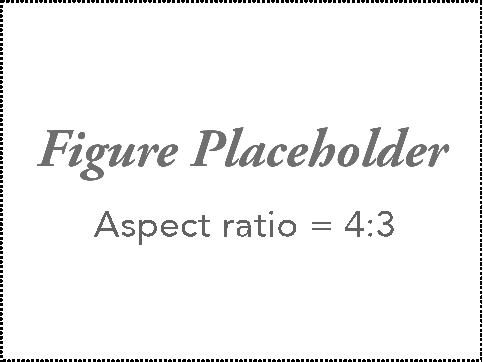
\includegraphics[width=5in]{draft4x3}
	\caption{Root-locus plot for stability modes.}
	\label{fig:stabilityeigen}
\end{figure}



\subsubsection{Mission Performance}
\label{sssec:missionperformance}



%----------------
%---   Estimated Mission Performance
%----------------
\begin{table}[h!]
	\centering
	\caption{Estimated Mission Performance.}
	\label{tab:estimatedmissionperformance}
	\rowcolors{2}{BYUbluelite}{white}
	\begin{tabular}{ C{1.5in}  C{1in}  C{1in}  C{1in}}
		
		\rowcolor{BYUbluemid}
		Parameter & Mission 1 & Mission 2 & Mission 3 \\
		
		Total Weight (lbs) & & &\\
		
		Wing Loading (lbs/ft\(^2\)) & & &\\
		
		\(V_C\)(ft/s) & & &\\
		
		\(V_{TO}\)(ft/s) & & &\\
		
		Payload & & &\\
		
		{\color{\BYUred} {\color{BYUred} [YEAR SPECIFIC ITEM]}} & & &\\
		
		Raw Mission Score & & &\\
		
	\end{tabular}
\end{table}